% =========================================================================
%  AtomSpect Theory Manual
%  Build:  make            (or: pdflatex AtomSpect_theory_manual.tex, twice)
%  Figures and tables are generated by scripts/make_figures.py
% =========================================================================
\documentclass[11pt,a4paper]{article}

\usepackage[utf8]{inputenc}
\usepackage[T1]{fontenc}
\usepackage{lmodern}
\usepackage{microtype}
\usepackage[a4paper,margin=2.5cm,headheight=14pt]{geometry}
\usepackage{amsmath,amssymb,mathtools}
\usepackage{graphicx}
\usepackage{booktabs,tabularx,longtable,array}
\usepackage{xcolor}
\usepackage{tikz}
\usetikzlibrary{arrows.meta,positioning,shapes.geometric,calc,fit,backgrounds}
\usepackage[font=small,labelfont=bf]{caption}
\usepackage{fancyhdr}
\usepackage[colorlinks=true,linkcolor=blue!50!black,citecolor=green!40!black,urlcolor=blue!50!black]{hyperref}

% ----------------------------------------------------------------- macros
\newcommand{\ket}[1]{\lvert #1\rangle}
\newcommand{\bra}[1]{\langle #1\rvert}
\newcommand{\braket}[2]{\langle #1\vert #2\rangle}
\newcommand{\mel}[3]{\langle #1\vert #2\vert #3\rangle}
\newcommand{\rme}[3]{\langle #1\Vert #2\Vert #3\rangle}
\newcommand{\vb}[1]{\boldsymbol{#1}}
\newcommand{\uv}[1]{\hat{\boldsymbol{#1}}}
\newcommand{\threej}[6]{\begin{pmatrix} #1 & #2 & #3\\ #4 & #5 & #6\end{pmatrix}}
\newcommand{\sixj}[6]{\begin{Bmatrix} #1 & #2 & #3\\ #4 & #5 & #6\end{Bmatrix}}
\newcommand{\code}[1]{\texttt{#1}}
\newcommand{\routine}[1]{\textsf{#1}}
\newcommand{\opt}[1]{\texttt{\detokenize{#1}}}
\newcommand{\doiurl}[1]{\href{https://doi.org/#1}{doi:#1}}
\newcommand{\dd}{\mathrm{d}}
\newcommand{\ii}{\mathrm{i}}
\newcommand{\ee}{\mathrm{e}}

\definecolor{notebg}{RGB}{243,247,252}
\definecolor{noteframe}{RGB}{42,111,176}
\definecolor{warnbg}{RGB}{253,245,236}
\definecolor{warnframe}{RGB}{217,130,43}
\newsavebox{\notebox}
\newenvironment{implnote}[1][Implementation]{%
  \par\smallskip\noindent\begin{lrbox}{\notebox}\setlength{\fboxsep}{6pt}\begin{minipage}{\dimexpr\linewidth-2\fboxsep-2\fboxrule\relax}\small\textbf{#1.}\ }{%
  \end{minipage}\end{lrbox}\setlength{\fboxsep}{6pt}\fcolorbox{noteframe}{notebg}{\usebox{\notebox}}\par\smallskip}
\newenvironment{caveat}[1][Caveat]{%
  \par\smallskip\noindent\begin{lrbox}{\notebox}\setlength{\fboxsep}{6pt}\begin{minipage}{\dimexpr\linewidth-2\fboxsep-2\fboxrule\relax}\small\textbf{#1.}\ }{%
  \end{minipage}\end{lrbox}\setlength{\fboxsep}{6pt}\fcolorbox{warnframe}{warnbg}{\usebox{\notebox}}\par\smallskip}

\numberwithin{equation}{section}
\setlength{\parindent}{0pt}
\setlength{\parskip}{0.55em}
\renewcommand{\arraystretch}{1.15}

\pagestyle{fancy}
\fancyhf{}
\fancyhead[L]{\small AtomSpect Theory Manual}
\fancyhead[R]{\small\nouppercase{\leftmark}}
\fancyfoot[C]{\small\thepage}
\renewcommand{\headrulewidth}{0.4pt}

\hypersetup{pdftitle={AtomSpect Theory Manual},pdfsubject={Zeeman and hyperfine spectra for plasma diagnostics}}

\newcommand{\muB}{\mu_{\mathrm B}}

\begin{document}
\hypersetup{pageanchor=false}

% ================================================================== title
\begin{titlepage}
\centering
\vspace*{3cm}
{\Huge\bfseries AtomSpect\par}
\vspace{0.6cm}
{\LARGE Theory Manual\par}
\vspace{0.4cm}
{\large Zeeman and hyperfine spectra for plasma diagnostics\par}
\vspace{2cm}
\begin{tabular}{rl}
Code version & 0.1.0.dev0 (development branch)\\
Code author & Leo Nofs\\
Manual date & October 2026
\end{tabular}
\vfill
\begin{minipage}{0.88\linewidth}
\raggedright\small
This manual describes the physics and numerical methods implemented in
AtomSpect: the within-term Zeeman Hamiltonian, hyperfine structure,
relative electric-dipole strengths, observation geometry, and continuous
line profiles. It states the conventions of the inputs and outputs and
cross-references the routines that implement each calculation. Numerical
checks run with the code itself are in Section~\ref{sec:validation}.
Known limitations are collected in Section~\ref{sec:limitations}; input
options are listed in Appendix~\ref{app:options}. The physical model is
presented in the AtomSpect paper, \doiurl{10.1016/j.jqsrt.2026.110015};
implementation conventions and departures are identified here.
\end{minipage}
\vspace{1.5cm}
\end{titlepage}

\pagenumbering{roman}
\hypersetup{pageanchor=true}
\begingroup
\setlength{\parskip}{0pt}
\tableofcontents
\endgroup
\clearpage
\pagenumbering{arabic}

% =========================================================================
\section{Introduction}\label{sec:intro}

AtomSpect computes relative electric-dipole (E1) spectra for a selected
lower and upper LS term in a static magnetic field, optionally including
hyperfine structure. The field splits and mixes the supplied levels;
every upper--lower eigenstate pair receives a wavelength, a relative
strength, and a polarization label. Doppler and instrumental profiles
turn the discrete (``stick'') spectrum into a continuous curve.

The model uses four principal steps:
\begin{enumerate}\setlength{\itemsep}{0pt}
  \item Field-free energies are supplied per $J$ level, lowest $J$ first;
        they are not calculated ab initio (Section~\ref{sec:units}).
  \item Clebsch--Gordan coefficients transform the angular-momentum
        operators into the coupled basis (Sections~\ref{sec:zeeman}
        and~\ref{sec:hfs}).
  \item Each isolated term is diagonalized separately, including the
        electronic and optional nuclear Zeeman interaction.
  \item E1 amplitudes between dressed states are weighted by the
        observation geometry, normalized, and broadened
        (Sections~\ref{sec:transitions}--\ref{sec:profile}).
\end{enumerate}
Radial matrix elements, level populations, collisional and Stark effects,
and absolute transition probabilities are outside this model. Strengths
sum to one when the detected signal is nonzero; a dark observation
returns zero strengths and a zero curve.

\subsection{Read this before running}
\begin{caveat}[Development version operating status]
The exact solver describes relative E1 spectra within isolated LS terms,
with optional hyperfine structure. Absolute rates and level populations
are absent. Approximation spectra with HFS are unavailable. Finite
convolution windows can lose broad wings or Doppler-shifted peaks;
check window and sampling convergence. See Section~\ref{sec:limitations}
for these restrictions and unvalidated research helpers.
\end{caveat}

The minimal example is \code{doc/scripts/example\_minimal.py}. It computes
He\,I 447\,nm sticks at 0.5\,T, reports their polarization labels, and
convolves them with a split Lorentzian. Optional plotting is enabled with
\code{--plot}. The returned \code{SpectrumResult} supports dictionary and
attribute access; \code{result.describe()} documents the result keys.

\subsection{Calculation flow}
Figure~\ref{fig:flow} shows the operations performed by
\routine{AtomSpect\_Main}; Table~\ref{tab:flowmap} maps them to the routines
and sections that explain each stage.

\clearpage
\begin{figure}[!htbp]
\centering
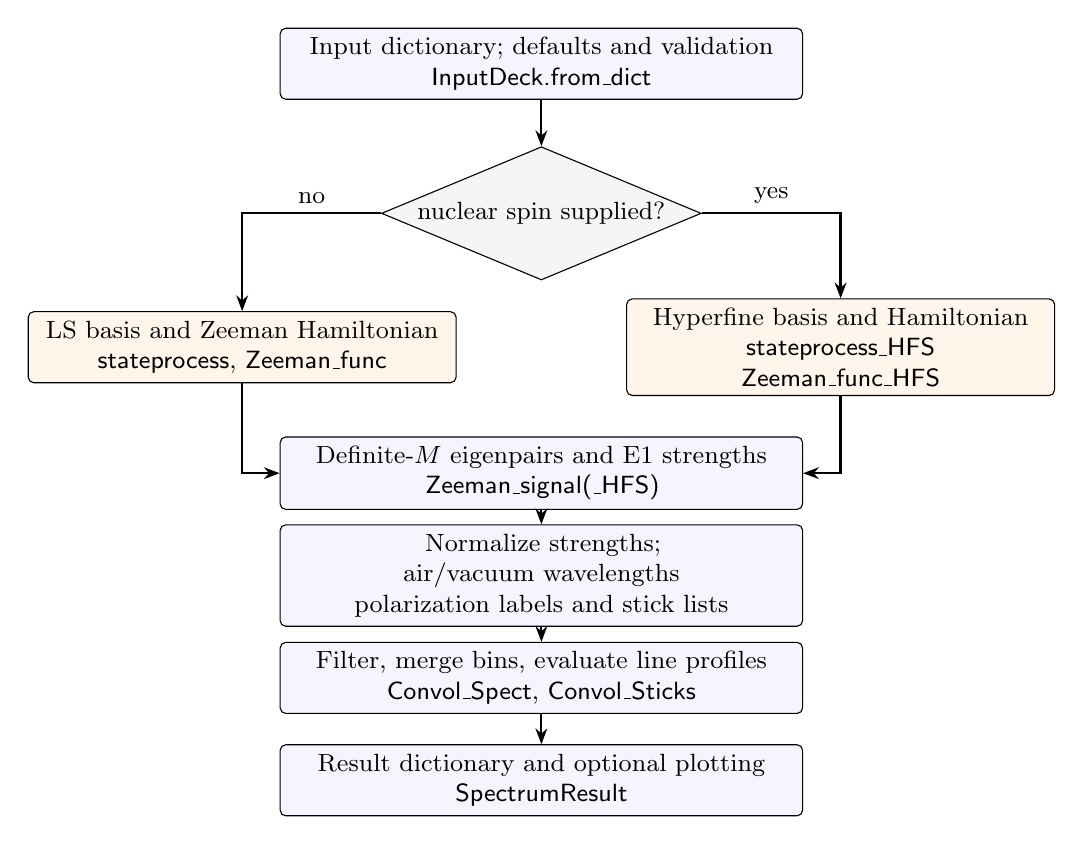
\begin{tikzpicture}[
  box/.style={draw,rounded corners=2pt,fill=blue!4,align=center,font=\small,minimum height=8mm,text width=64mm},
  sbox/.style={draw,rounded corners=2pt,fill=orange!8,align=center,font=\small,minimum height=8mm,text width=52mm},
  dec/.style={draw,diamond,aspect=2.4,fill=gray!8,align=center,font=\small,inner sep=1pt},
  arr/.style={-{Stealth[length=2mm]},thick}]
\node[box] (in) at (0,0) {Input dictionary; defaults and validation\\ \routine{InputDeck.from\_dict}};
\node[dec] (mode) at (0,-1.9) {nuclear spin supplied?};
\node[sbox] (fine) at (-3.8,-3.6) {LS basis and Zeeman Hamiltonian\\ \routine{stateprocess}, \routine{Zeeman\_func}};
\node[sbox] (hfs) at (3.8,-3.6) {Hyperfine basis and Hamiltonian\\ \routine{stateprocess\_HFS}\\ \routine{Zeeman\_func\_HFS}};
\node[box] (dip) at (0,-5.2) {Definite-$M$ eigenpairs and E1 strengths\\ \routine{Zeeman\_signal(\_HFS)}};
\node[box] (sticks) at (0,-6.5) {Normalize strengths; air/vacuum wavelengths\\ polarization labels and stick lists};
\node[box] (cont) at (0,-7.8) {Filter, merge bins, evaluate line profiles\\ \routine{Convol\_Spect}, \routine{Convol\_Sticks}};
\node[box] (out) at (0,-9.1) {Result dictionary and optional plotting\\ \routine{SpectrumResult}};
\draw[arr] (in)--(mode);
\draw[arr] (mode)-|node[above,pos=.25,font=\small]{no}(fine);
\draw[arr] (mode)-|node[above,pos=.25,font=\small]{yes}(hfs);
\draw[arr] (fine)|-(dip); \draw[arr] (hfs)|-(dip);
\draw[arr] (dip)--(sticks); \draw[arr] (sticks)--(cont); \draw[arr] (cont)--(out);
\end{tikzpicture}
\caption{Calculation flow of \routine{AtomSpect\_Main}. Optional weak- and
high-field spectra use separate non-HFS solves; energy fans sweep the
Hamiltonian over field samples. Neither branch supplies absolute rates.}
\label{fig:flow}
\end{figure}

\begin{table}[!htbp]
\centering\small
\begin{tabularx}{\textwidth}{>{\raggedright\arraybackslash}p{4.2cm}>{\raggedright\arraybackslash}X r}
\toprule
Step & Routines & Section\\
\midrule
Defaults and input handling & \routine{InputDeck.from\_dict} & \ref{sec:usage}\\
LS basis and Zeeman structure & \routine{stateprocess}, \routine{Zeeman\_func} & \ref{sec:zeeman}\\
Hyperfine structure & \routine{stateprocess\_HFS}, \routine{Zeeman\_func\_HFS} & \ref{sec:hfs}\\
Angular E1 amplitudes & \routine{dipolestr}, \routine{dipolestr\_HFS} & \ref{sec:transitions}\\
Observation geometry & \routine{polarization} & \ref{sec:pol}\\
Eigenpair strengths & \routine{Zeeman\_signal}, \routine{Zeeman\_signal\_HFS} & \ref{sec:transitions}\\
Continuous profile & \routine{make\_stickbins}, \routine{Convol\_Spect} & \ref{sec:profile}\\
Energy fans & \routine{ZeemanFan}, \routine{FastZfan} & \ref{sec:zeeman}, \ref{sec:hfs}\\
Numerical checks & \code{scripts/make\_figures.py}, repository tests & \ref{sec:validation}\\
\bottomrule
\end{tabularx}
\caption{Where each part of the calculation is implemented and documented.}
\label{tab:flowmap}
\end{table}

\subsection{Units and conventions}\label{sec:units}
\begin{center}\small
\begin{tabularx}{\textwidth}{>{\raggedright\arraybackslash}p{4.2cm}>{\raggedright\arraybackslash}p{3.6cm}>{\raggedright\arraybackslash}X}
\toprule
Quantity & Unit & Note\\
\midrule
Level energies, term energies & cm$^{-1}$ & lowest $J$ first\\
Magnetic field $B$ & T & \\
Wavelengths & nm & air wavelengths by default; vacuum also returned\\
Hyperfine constants $A$, $B$ & Hz & converted with $1/(100\,c)$\\
Temperature & K (\code{Temp}) or eV (\code{TempeV}) & $1\,\mathrm{eV}=11602$ K\\
Line-profile functions & m & called with nm values scaled by $10^{-9}$\\
\bottomrule
\end{tabularx}
\end{center}

\paragraph{Constants.} $g_L=1$, $g_S=2.002319$, $\muB=0.466868$~cm$^{-1}$T$^{-1}$ (from $5.7883818\times10^{-5}$~eV/T and $1.23981\times10^{-4}$~eV$\cdot$cm). The nuclear $g$ factor is $g_I=(\mu_I/I)(m_e/m_p)$ with $\mu_I$ in nuclear magnetons.

\paragraph{Spin input.} The keys \code{s\_ground} and \code{s\_excited} are the spin quantum numbers $S$, not the multiplicities $2S+1$: a triplet is entered as $S=1$.

% ------------------------------------------------------------------------
\section{Zeeman structure}\label{sec:zeeman}

For a term with quantum numbers $L,S$, the code stores paired labels $[J,m_J,L,m_L,S,m_S]$, with $J=\vert L-S\vert,\dots,L+S$, built from the Clebsch--Gordan coefficients $\langle L m_L S m_S\vert J m_J\rangle$. These coefficients form the matrix $\Psi$ that transforms between the coupled and uncoupled bases. The zero-field Hamiltonian is diagonal, $H_0=\mathrm{diag}(E_J)$, with $E_J$ repeated for the $2J+1$ values of $m_J$.

\subsection{Intermediate field (exact within the term)}
\begin{equation}
H = H_0 + \muB B\,\bigl(g_S S_z + g_L L_z\bigr),\qquad
S_z \to \Psi\,\mathrm{diag}(m_S)\,\Psi^{T},\quad L_z \to \Psi\,\mathrm{diag}(m_L)\,\Psi^{T}.
\end{equation}
$H$ is diagonalized numerically. The eigenvectors are expressed in the coupled basis. Because $S_z+L_z$ conserves $m_J$, $m_J$ remains a good quantum number at every field, while $J$ mixes.

\begin{implnote}
\routine{stateprocess} constructs the basis transformation;
\routine{Zeeman\_func} diagonalizes the Hamiltonian. \routine{HZeeman}
returns the unscaled Zeeman operator for repeated field solves. Multiply
it by $\muB B$ before adding it to the zero-field energy matrix.
\end{implnote}

\subsection{Low-field approximation}
When $\muB B\ll$ the fine-structure splittings, $E=E_J+g_J m_J\muB B$ with
\begin{equation}
g_J = g_L\frac{J(J+1)-S(S+1)+L(L+1)}{2J(J+1)} + g_S\frac{J(J+1)+S(S+1)-L(L+1)}{2J(J+1)},\qquad g_{J=0}=0 .
\end{equation}
The electron $g$ factors are the same as in the exact Hamiltonian, so the exact result approaches this one at weak field. Fan rows follow ascending energy rank at each sample; individual states are not tracked through level crossings.

\subsection{High-field (Paschen--Back) approximation}
When $\muB B$ is much larger than the fine-structure splittings, the levels are $E=E_{\mathrm{term}}+\muB B\,(g_L m_L+g_S m_S)$, diagonal in the uncoupled basis; the eigenvectors are rotated back to the coupled basis with $\Psi$. This regime requires the term energy $E_{\mathrm{term}}$ (\code{EtermG}, \code{EtermE}) and neglects fine structure.

\begin{caveat}
The high-field approximation uses the ideal $g_S=2$ of the uncoupled expression and ignores fine structure entirely. It is an asymptotic illustration, not a substitute for the exact intermediate-field result. In the driver it produces strengths and wavelengths only; its polarization labels are not resolved by eigenstate pair.
\end{caveat}

\begin{figure}[!htbp]
\centering
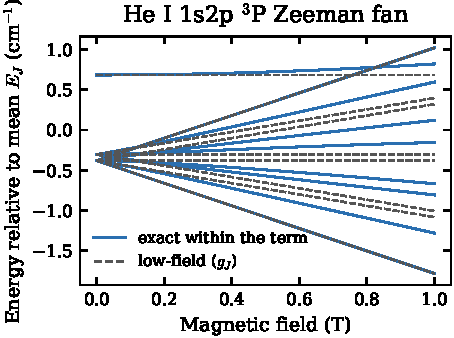
\includegraphics[width=0.5\textwidth]{figures/fig_zeeman_fan.pdf}
\caption{Zeeman fan of the He\,I 1s2p $^3$P term (inputs from the repository example). The exact levels (solid) approach the $g_J$ low-field lines (dashed) at weak field and mix $J$ near 1\,T.}
\end{figure}

% ------------------------------------------------------------------------
\section{Hyperfine structure}\label{sec:hfs}

With nuclear spin $I$ the bookkeeping lists are $[F,m_F,J,m_J,I,m_I,L,m_L,S,m_S]$, with bases related by two successive couplings, $(L,S)\to J$ and $(J,I)\to F$; the matrix $\Psi$ is the product of the two Clebsch--Gordan matrices.

\subsection{Zero-field hyperfine energies}
With $K=F(F+1)-I(I+1)-J(J+1)$, the shift of a level of a given $J$ is
\begin{equation}
\Delta E_{\mathrm{hfs}} = \frac{A K}{2}
 + B\,\frac{\tfrac34 K(K+1)-I(I+1)J(J+1)}{2I(2I-1)J(2J-1)},
\end{equation}
and the quadrupole term is set to zero when $I\le\tfrac12$, $J\le\tfrac12$ or $B=0$. $A$ and $B$ are given per $J$ level in Hz and converted to cm$^{-1}$. This diagonal term is added to $H_0$ in the $\vert F,m_F\rangle$ basis.

\subsection{Zeeman Hamiltonian with hyperfine structure}
\begin{equation}
H = H_0 + H_{\mathrm{hfs}} + \muB B\,\bigl(g_S S_z + g_L L_z - g_I I_z\bigr),
\end{equation}
diagonalized exactly. Here the full $\Psi$ transformation projects $S_z$, $L_z$ and $I_z$ into the coupled basis. The projected operators conserve $m_F$.

\begin{implnote}
\routine{stateprocess\_HFS} assigns the supplied $A$ and $B$ constants
per $J$ level. \routine{Zeeman\_func\_HFS} includes their diagonal shifts
and the electronic and nuclear Zeeman operators. The legacy
\opt{PsiHFS} input does not select a different Hamiltonian.
\end{implnote}

\subsection{Weak-field hyperfine approximation (fans only)}
Projecting the electronic and nuclear operators onto $\vert F,m_F\rangle$ gives
\begin{equation}
g_F = g_J\frac{F(F+1)-I(I+1)+J(J+1)}{2F(F+1)}
      -g_I\frac{F(F+1)+I(I+1)-J(J+1)}{2F(F+1)},\qquad g_{F=0}=0.
\end{equation}
The shift is $g_F m_F\muB B$. The nuclear minus sign is shared with the exact Hamiltonian. A spin-zero nucleus has zero magnetic moment and $g_I=0$.

\subsection{Hyperfine Paschen--Back approximation (fans only)}
For field sweeps, \code{ZeemanFan} can also return an approximation in which $J$ is kept and $I_z$ and $J_z$ decouple: each diagonal element is the sum of the fine-structure energy, the $A$ and $B$ hyperfine terms evaluated for the uncoupled projections, and the electronic and nuclear Zeeman terms (with the nuclear sign above).

\begin{figure}[!htbp]
\centering
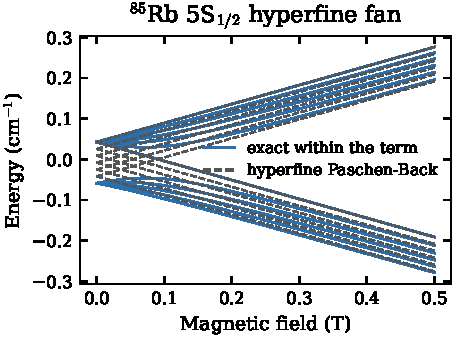
\includegraphics[width=0.5\textwidth]{figures/fig_hfs_fan.pdf}
\caption{$^{85}$Rb 5S$_{1/2}$ hyperfine fan. At $B=0$ the two manifolds are separated by $A(I+\tfrac12)$; the approximation (dashed) is accurate once the Zeeman energy dominates the hyperfine splitting.}
\end{figure}

\begin{caveat}
Spectra with the low- or high-field approximation are not implemented with hyperfine structure; enabling \code{DoLowSig} or \code{DoHighSig} with \code{I\_spin} raises \code{NotImplementedError}. The hyperfine constants and the nuclear moment are inputs and are not validated against tables by the code.
\end{caveat}

% ------------------------------------------------------------------------
\section{Transition strengths}\label{sec:transitions}

\subsection{Basis-pair dipole factors}
Without hyperfine structure the reduced dipole factor between a lower state $\vert J,m_J,L,\dots\rangle$ and an upper state $\vert J',m_J',L',S,\dots\rangle$ (Metcalf, Eq.~4.32) is
\begin{equation}
d = (-1)^{L'+S-m_J'}\sqrt{(2J'+1)(2J+1)}\;\threej{J}{1}{J'}{m_J}{q}{-m_J'}\sixj{L'}{J'}{S}{J}{L}{1},\qquad q=m_J'-m_J .
\end{equation}
Without hyperfine structure the code evaluates this expression with the roles of the two states exchanged; that changes only a sign that is common to all pairs of one $q$ channel, and so drops out of the squared amplitude of a definite-$M$ eigenpair. With hyperfine structure (Metcalf, Eq.~4.33) the factor contains two $6j$ symbols, one for the $F$--$J$ coupling and one for the $J$--$L$ coupling:
\begin{multline}
d = (-1)^{1+L'+S+J+J'+I-m_F'}\sqrt{(2F+1)(2F'+1)(2J+1)(2J'+1)}\\
\times\threej{F}{1}{F'}{m_F}{q}{-m_F'}\sixj{L'}{J'}{S}{J}{L}{1}\sixj{J'}{F'}{I}{F}{J}{1}.
\end{multline}
The $3j$ and $6j$ symbols come from \code{sympy}. The code does not include the radial integral, so only ratios of strengths are meaningful.

\subsection{Eigenpair amplitudes and normalization}
Let $c^{u}$ and $c^{l}$ be the eigenvector matrices of the upper and lower level, and let $\mathcal A=c^{u*}\otimes c^{l}$ (a Kronecker product, lower index fastest). For every basis pair $p$ the coefficient is $s_p=\epsilon_{q_p}\,d_p$, where $\epsilon_q$ is the polarization amplitude of Section~\ref{sec:pol}. The strength of eigenpair $k$ is
\begin{equation}
I_k=\Bigl\vert\sum_p \mathcal A_{pk}\,s_p\Bigr\vert^{2},\qquad \hat I_k=\frac{I_k}{\sum_{k'} I_{k'}},
\end{equation}
so that the reported \code{signal} sums to one if the denominator is nonzero. When both transmissions vanish, the strengths remain zero instead of dividing by zero. The wavelength follows from the eigenvalues, $\lambda_{\mathrm{vac}}=10^{7}/(E_u-E_l)$ nm, and the air wavelength from the standard vacuum-to-air relation.

\begin{caveat}
Quantities such as \code{A\_Ein}, \code{f\_osc} and \code{S\_line} are not valid absolute radiative quantities: without a radial matrix element, a normalized angular strength cannot give a transition probability. They are therefore only returned on request (\code{RadiativePlaceholders}), together with a warning. Their $2J'+1$ normalization is also tied to the basis-state list, not to field-mixed states.
\end{caveat}

% ------------------------------------------------------------------------
\begin{implnote}
\routine{Zeeman\_signal} and \routine{Zeeman\_signal\_HFS} form
relative strengths and wavelengths. The internal definite-$M$ solver
resolves polarization labels for exact spectra. Returned basis-pair
lists remain bookkeeping arrays; they are not labels of the dressed
eigenstates.
\end{implnote}

\section{Polarization}\label{sec:pol}

Following Isler (1997), with $\theta$ the angle between the magnetic field and the line of sight and $\gamma$ the angle of an optional linear polarizer measured from the $\pi$ axis,
\begin{align}
e_\alpha &= \sqrt{T_\alpha}\cos\gamma, & e_\beta &= \sqrt{T_\beta}\sin\gamma && (\text{filter present}),\\
e_\alpha &= \sqrt{T_\alpha}, & e_\beta &= \sqrt{T_\beta} && (\text{no filter}),\\
\epsilon_{0} &= e_\alpha\sin\theta, &
\epsilon_{\pm1} &= \sqrt{\tfrac12\bigl(e_\alpha^{2}\cos^{2}\theta+e_\beta^{2}\bigr)} .
\end{align}
$T_\alpha$, $T_\beta$ (\code{TAlpha}, \code{TBeta}) describe transmission of other optics and default to one. A pair is labelled by $q=M_u-M_l$: $q=0$ is $\pi$ light, $q=\pm1$ is $\sigma$ light, and any other value has no E1 component and is labelled 3. The public stick lists keep the emitted-light sign convention, so \code{sigmaplus\_sticks} collects $q=-1$.

\paragraph{Labels belong to eigenstate pairs.} $M$ ($m_J$, or $m_F$ with hyperfine structure) is a good quantum number, so each eigenvector has a definite $M$. The code rebuilds the Hamiltonian from the eigensystem, diagonalizes each $M$ block separately, and labels every eigenpair with the exact $M$ of its two eigenvectors. Labelling the basis pairs instead, which an earlier version did, assigns false $\pi/\sigma$ labels once states mix. Equal-energy eigenvectors may be replaced by a reconstructed basis, so the identity of an individual coincident line is not preserved; only the summed strength of coincident lines has meaning.

\begin{figure}[!htbp]
\centering
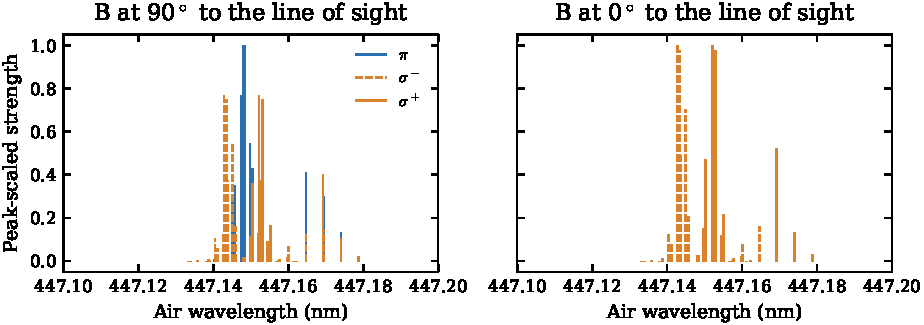
\includegraphics[width=0.92\textwidth]{figures/fig_polarization.pdf}
\caption{He\,I 447\,nm sticks at 0.5\,T split by polarization. Blue denotes $\pi$; orange denotes $\sigma$, solid for $\sigma^+$ and dashed for $\sigma^-$. With the field perpendicular to the line of sight all three kinds are visible; along the field the $\pi$ light vanishes.}
\end{figure}

% ------------------------------------------------------------------------
\section{Continuous line profile}\label{sec:profile}

Sticks are convolved with unit-area profiles in metres. The instrument
width \opt{pixel_size} is a full width at half maximum; the input key
\opt{specstep} supplies it in nm. The pure Doppler Gaussian has no
instrument-width argument, but uses \opt{specstep} to set its sampling
scale.

\begin{center}\small
\begin{tabularx}{\textwidth}{>{\raggedright\arraybackslash}p{3.1cm}>{\raggedright\arraybackslash}X}
\toprule
Name & Definition\\
\midrule
\code{Gaussian} & Doppler: $\sigma=\lambda_0\sqrt{k_BT/(Mc^2)}$, mean $\lambda_0(1+v/c)$.\\
\code{GaussianInstrum} & Gaussian with FWHM $W=\sqrt{\mathrm{pix}^2+8\ln2\,\sigma^2}$ (instrument and Doppler in quadrature).\\
\code{Voigt} & Doppler $\sigma$ convolved with a Lorentzian of FWHM \code{pixel\_size} (HWHM $=$ pix$/2$ for \code{scipy}).\\
\code{Lorrentzian}, \code{Skewed} & Symmetric Lorentzian, or split Lorentzian with half widths $s_{L,R}\,\mathrm{pix}/2$ for \code{Skewed}; unit area.\\
\bottomrule
\end{tabularx}
\end{center}

Ion motion shifts the mean by $\lambda_0 v/c$; with \code{bidir} the profile is the average of the $\pm v$ components. All profiles integrate to one, so the total strength of a stick does not depend on the profile choice (Fig.~\ref{fig:shapes}).

\begin{figure}[!htbp]
\centering
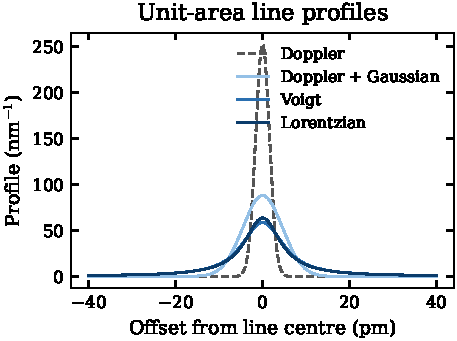
\includegraphics[width=0.5\textwidth]{figures/fig_lineshapes.pdf}
\caption{Unit-area profiles at 600\,nm for a 3000\,K, mass-40 emitter and a 10\,pm instrument width.}\label{fig:shapes}
\end{figure}

\paragraph{Binning and truncation.} For speed, neighbouring sticks separated by at most $2\,\code{fxnwindow}$ (nm) share a bin, merging overlapping padded windows, and each bin is evaluated only within \code{fxnwindow} of its outermost sticks, at \code{specres} points per pixel. Components at or below $0.05\,\max/N$ are dropped. The grid includes the bin endpoints and uses at least two samples; its spacing is approximately \code{specstep}/\code{specres}. The Lorentzian tail beyond $\pm w$ carries the fraction $1-\tfrac{2}{\pi}\arctan(w/\gamma)$ of a symmetric line's area ($\gamma$ the HWHM); the input check warns when this exceeds 2\%. For Voigt this reports only the Lorentzian-tail estimate, not the total finite-window loss.

\paragraph{Density units.} \code{SpecOut} has a wavelength axis in nm but retains profile values per metre. Its integral against the nm axis is therefore $10^9$ times its integral against metres. For a density per nm, multiply the vertical values by $10^{-9}$. Sampling, filtering and finite windows can reduce the captured area; the plotted curve is not renormalized.

\begin{caveat}
Binning and the \code{spec\_window} filter use rest wavelengths. Large ion velocities can move a profile centre beyond its padded bin, so increase \code{fxnwindow} and the physics window for such cases. The code does not adapt windows to the Doppler shift or enforce convergence. Gaussian tails can also be truncated without a warning. The first-order Doppler shift assumes $|v|\ll c$.
\end{caveat}

% ------------------------------------------------------------------------
\begin{implnote}
\routine{make\_stickbins} merges overlapping padded intervals;
\routine{Convol\_Sticks} evaluates a unit-area profile within each
interval; \routine{Convol\_Spect} weights and sums the curves. The
wavelength axis is in nm while profile density remains per metre.
\end{implnote}

\section{Using AtomSpect}\label{sec:usage}

\paragraph{Input.} \code{AtomSpect\_Main} takes a dictionary. The required keys are \code{s\_ground}, \code{s\_excited}, \code{l\_ground}, \code{l\_excited}, \code{E\_ground}, \code{E\_excited}, \code{Bmag} and \code{b\_angle}. Unknown keys raise a warning with a suggestion. Level energies must match the allowed $J$ values, lowest $J$ first; HFS constants may be scalars or one per $J$. Widths, masses and sampling factors must be positive, and optical transmissions nonnegative. A pure Gaussian requires positive temperature. The Gaussian, \code{GaussianInstrum} and Voigt profiles need \code{Temp} or \code{TempeV}. The full list with defaults is in \code{AtomSpect\_Main}'s docstring and in the README.

\paragraph{Output.} The result is a dictionary with attribute access. Its type is \routine{SpectrumResult}; call \code{result.describe()} for descriptions of its entries. Principal entries include \opt{signal} and \opt{wave_air} for the sticks, \opt{rad} for polarization labels, and \opt{SpecOut} for the continuous curve. Separate \code{pi}/\code{sigma} stick lists are also returned. \code{ZeemanSplits\_G} is now a vector of lower-level energies in cm$^{-1}$; earlier code accidentally returned the eigenvector matrix. Exact basis metadata is retained when approximation spectra are also requested.

\begin{table}[!htbp]
\centering\small
\begin{tabular}{ll}
\toprule
Module & Contents\\
\midrule
\code{constants}, \code{units} & constants; energy and wavelength conversions\\
\code{angular} & $g$ factors, Clebsch--Gordan and $3j/6j$ wrappers, dipole factors\\
\code{levels} & state lists and coupling matrices\\
\code{hamiltonian}, \code{hfs} & Zeeman and hyperfine Hamiltonians, eigenvector resolution\\
\code{polarization}, \code{transitions} & polarization amplitudes and labels; strengths and wavelengths\\
\code{fan} & energy fans versus $B$\\
\code{lineshapes}, \code{convolution} & profiles; binning and convolution\\
\code{config}, \code{spectrum}, \code{result} & input validation; the driver; the result class\\
\code{plotting}, \code{io} & plots and the slider GUI; reading and saving data\\
\bottomrule
\end{tabular}
\caption{Module map of the AtomSpect package.}
\end{table}

% ------------------------------------------------------------------------
\section{Numerical validation}\label{sec:validation}

\subsection{Analytic checks}
The script \code{scripts/make\_figures.py} evaluates the checks in Table~\ref{tab:checks} before writing any figure and aborts if one fails. They test specific limits of the implemented model; they do not establish the correctness of the whole code or its agreement with experiment.

\begin{table}[!htbp]
\centering\small
\begin{tabular}{lcc}
\toprule
Check & measured & tolerance \\
\midrule
\texttt{weak\_field\_zeeman\_3P2\_cm-1} & 8.73e-11 & 1e-09 \\
\texttt{rb85\_5S\_hyperfine\_interval\_relative} & 1.37e-16 & 1e-09 \\
\texttt{strength\_normalization} & 0.00e+00 & 1e-12 \\
\texttt{no\_forbidden\_components} & 0.00e+00 & 1e-14 \\
\texttt{pi\_strength\_along\_field} & 0.00e+00 & 1e-12 \\
\texttt{gaussian\_unit\_area} & 0.00e+00 & 1e-03 \\
\texttt{voigt\_unit\_area} & 7.96e-04 & 1e-03 \\
\texttt{lorentzian\_fwhm\_m} & 7.37e-23 & 2e-14 \\
\texttt{hfs\_weak\_field\_projection} & 4.44e-16 & 1e-12 \\
\texttt{overlapping\_bin\_profile\_sum} & 3.81e-16 & 1e-12 \\
\texttt{dark\_spectrum\_strength} & 0.00e+00 & 0e+00 \\
\bottomrule
\end{tabular}

\caption{Analytic checks: weak-field splitting of $^3$P$_2$ against $g_J m \muB B$ (absolute, cm$^{-1}$); $^{85}$Rb 5S hyperfine interval against $A(I+\tfrac12)$ (relative); normalization; absence of $\lvert\Delta M\rvert>1$ strength; vanishing $\pi$ light along the field; profile areas and widths; weak-field HFS projection; overlapping-bin profile summation; a dark observation.}\label{tab:checks}
\end{table}

The repository's test suite adds regression tests for the polarization labels (with and without hyperfine structure), the high-field and fan approximations, the Boolean approximation flags, the profiles and a set of golden outputs for refactoring.

\section{Known limitations and implementation notes}\label{sec:limitations}
\begin{itemize}\setlength\itemsep{0pt}
\item Only relative strengths are meaningful. No radial matrix elements, populations or photon-energy weighting.
\item Each term is isolated. Mixing between terms of different $L$ or $S$ and configuration interaction are not modelled.
\item Hyperfine constants and moments are user inputs. The estimator module \code{hfs\_estimate} (semi-empirical A and B constants) is a research aid. Its B-constant routines evaluate $B=eQV_{zz}$ in SI units; the underlying hydrogenic A-constant model is pinned by tests but not validated.
\item The non-HFS high-field approximation neglects fine structure and uses $g_S=2$.
\item \code{sortE} changes only the order in which basis states are listed, not the eigenvalues, and is slow.
\item Without \code{Convfxn} the symmetric Lorentzian is used and \code{Temp} is ignored. \code{Skewness} is used only by \code{Skewed}.
\item The inverse air-to-vacuum helper evaluates the refractive index at the air wavelength. It is an approximation, not an exact inverse; arbitrary wavelength ranges are not validated.
\item \code{Calc\_HFS\_Vals} is a reserved input and does not estimate missing constants.
\item The legacy \code{Zsig\_norad} helper retains raw eigenvectors; individual values can depend on the basis chosen in degenerate subspaces. Use the labelled spectrum for polarization-resolved results.
\end{itemize}

\subsection{Reproducing this manual}
From the repository root, run:
\begin{verbatim}
python doc/scripts/example_minimal.py
python -m pytest -q
python doc/scripts/make_figures.py --data-only
python doc/scripts/plot_figures.py
python doc/scripts/build_manual.py
\end{verbatim}
The data generator stages output until all checks and calculations succeed. The plotting script redraws all four PDFs from the CSV files. Provenance records UTC time, runtime versions, source commit, a source-content hash, and figure settings. Add \code{--rebuild} to the manual builder to regenerate data and figures before compiling. The Makefile offers equivalent data, plots, figures, check and rebuild targets. LaTeX failures stop the build.

\appendix
\clearpage
\section{Options and physical parameters}\label{app:options}

Required entries are marked with a dash. Both terms use the same unit
and ordering conventions. Full result-key descriptions are available from
\code{result.describe()}.

\begingroup\footnotesize
\begin{longtable}{>{\raggedright\arraybackslash}p{5.6cm}>{\raggedright\arraybackslash}p{2.5cm}>{\raggedright\arraybackslash}p{6.6cm}}
\toprule
Input & Default & Meaning (symbol, section)\\
\midrule\endhead
\opt{s_ground}/\opt{s_excited} & --- & spin $S$, not $2S+1$ (\S\ref{sec:units})\\
\opt{l_ground}/\opt{l_excited} & --- & orbital angular momentum $L$ (\S\ref{sec:zeeman})\\
\opt{E_ground}/\opt{E_excited} & --- & one energy per $J$ in cm$^{-1}$, lowest $J$ first\\
\opt{Bmag} & --- & scalar field [T]; field array for fans\\
\opt{b_angle} & --- & angle between field and line of sight [degrees] (\S\ref{sec:pol})\\
\opt{Pol_angle} & absent & linear analyzer angle [degrees]; zero enables the filter\\
\opt{TAlpha}/\opt{TBeta} & 1 / 1 & nonnegative intensity transmissions\\
\opt{amu} & 1 & emitter mass number\\
\opt{Convfxn} & \code{Lorrentzian} & Gaussian, GaussianInstrum, Voigt, Skewed, or symmetric Lorentzian (\S\ref{sec:profile})\\
\opt{Temp}/\opt{TempeV} & profile-dependent & temperature [K]/[eV]; eV takes precedence; required for thermal profiles\\
\opt{specstep} & 0.002222 nm & instrument FWHM and sampling pixel width; 0.002 nm if \opt{Convfxn} is supplied\\
\opt{specres} & 10 & nominal samples per pixel\\
\opt{fxnwindow} & 0.1 nm & padding of rest-wavelength bins (\S\ref{sec:profile})\\
\opt{Skewness} & [1,1] & left/right half-width multipliers, only for Skewed\\
\opt{ion_vel} & 0 & velocity [m/s]; scalar or counterstreaming pair\\
\opt{bidir} & False & average $+v$ and $-v$, or $+v_1$ and $-v_2$\\
\opt{SpectrumData} & absent & measured [wavelengths in nm, intensities]\\
\opt{spec_window}/\opt{plot_window} & [1,1000] nm & physics/plot bounds; default to measured wavelength range when supplied\\
\opt{I_spin} & absent & nuclear spin $I$; enables HFS (\S\ref{sec:hfs})\\
\opt{mu_I} & required with HFS & nuclear magnetic moment [nuclear magnetons]\\
\opt{HFS_G}/\opt{HFS_E} & required with HFS & dipole $A$ constants [Hz], scalar or one per $J$\\
\opt{HFSB_G}/\opt{HFSB_E} & 0 & quadrupole $B$ constants [Hz], scalar or one per $J$\\
\opt{PsiHFS} & False & legacy setting; same Hamiltonian for both values\\
\opt{Calc_HFS_Vals} & ignored & reserved; no constant estimation\\
\opt{DoLowSig}/\opt{DoHighSig} & False / False & non-HFS approximation spectra; Boolean or yes/no values\\
\opt{EtermG}/\opt{EtermE} & absent & term energies [cm$^{-1}$] for non-HFS high-field solves; zero is valid\\
\opt{sortE} & False & order approximation bases by weak-field energy\\
\opt{RadiativePlaceholders} & False & opt-in unvalidated legacy radiative outputs (\S\ref{sec:limitations})\\
\opt{plottitle} & absent & plotting title\\
\bottomrule
\end{longtable}
\endgroup

% =========================================================================
\clearpage
\begin{thebibliography}{99}
\bibitem{isler} R.\,C.\ Isler, Phys.\ Plasmas \textbf{4}, 3 (1997),
  \doiurl{10.1063/1.872095} (polarization of Zeeman components).
\bibitem{metcalf} H.\,J.\ Metcalf and P.\ van der Straten,
  \emph{Laser Cooling and Trapping}, Eqs.\ 4.32--4.33 (dipole factors).
\bibitem{steck} D.\,A.\ Steck, \emph{Rubidium 85 D Line Data},
  \url{https://steck.us/alkalidata/} (hyperfine constants and structure).
\bibitem{stone} N.\,J.\ Stone, At.\ Data Nucl.\ Data Tables \textbf{90},
  75 (2005), \doiurl{10.1016/j.adt.2005.04.001} (nuclear moments).
\bibitem{kopfermann} H.\ Kopfermann, \emph{Nuclear Moments}
  (hyperfine interaction).
\bibitem{nofs} L.\ Nofs \emph{et al.}, J.\ Quant.\ Spectrosc.\ Radiat.\
  Transf.\ (2026), \doiurl{10.1016/j.jqsrt.2026.110015}
  (the AtomSpect paper).
\end{thebibliography}

\end{document}
